\documentclass[]{book}
\usepackage{lmodern}
\usepackage{amssymb,amsmath}
\usepackage{ifxetex,ifluatex}
\usepackage{fixltx2e} % provides \textsubscript
\ifnum 0\ifxetex 1\fi\ifluatex 1\fi=0 % if pdftex
  \usepackage[T1]{fontenc}
  \usepackage[utf8]{inputenc}
\else % if luatex or xelatex
  \ifxetex
    \usepackage{mathspec}
  \else
    \usepackage{fontspec}
  \fi
  \defaultfontfeatures{Ligatures=TeX,Scale=MatchLowercase}
\fi
% use upquote if available, for straight quotes in verbatim environments
\IfFileExists{upquote.sty}{\usepackage{upquote}}{}
% use microtype if available
\IfFileExists{microtype.sty}{%
\usepackage{microtype}
\UseMicrotypeSet[protrusion]{basicmath} % disable protrusion for tt fonts
}{}
\usepackage[margin=1in]{geometry}
\usepackage{hyperref}
\hypersetup{unicode=true,
            pdftitle={life's work},
            pdfauthor={Charles T. Gray},
            pdfborder={0 0 0},
            breaklinks=true}
\urlstyle{same}  % don't use monospace font for urls
\usepackage{natbib}
\bibliographystyle{apalike}
\usepackage{color}
\usepackage{fancyvrb}
\newcommand{\VerbBar}{|}
\newcommand{\VERB}{\Verb[commandchars=\\\{\}]}
\DefineVerbatimEnvironment{Highlighting}{Verbatim}{commandchars=\\\{\}}
% Add ',fontsize=\small' for more characters per line
\usepackage{framed}
\definecolor{shadecolor}{RGB}{248,248,248}
\newenvironment{Shaded}{\begin{snugshade}}{\end{snugshade}}
\newcommand{\AlertTok}[1]{\textcolor[rgb]{0.94,0.16,0.16}{#1}}
\newcommand{\AnnotationTok}[1]{\textcolor[rgb]{0.56,0.35,0.01}{\textbf{\textit{#1}}}}
\newcommand{\AttributeTok}[1]{\textcolor[rgb]{0.77,0.63,0.00}{#1}}
\newcommand{\BaseNTok}[1]{\textcolor[rgb]{0.00,0.00,0.81}{#1}}
\newcommand{\BuiltInTok}[1]{#1}
\newcommand{\CharTok}[1]{\textcolor[rgb]{0.31,0.60,0.02}{#1}}
\newcommand{\CommentTok}[1]{\textcolor[rgb]{0.56,0.35,0.01}{\textit{#1}}}
\newcommand{\CommentVarTok}[1]{\textcolor[rgb]{0.56,0.35,0.01}{\textbf{\textit{#1}}}}
\newcommand{\ConstantTok}[1]{\textcolor[rgb]{0.00,0.00,0.00}{#1}}
\newcommand{\ControlFlowTok}[1]{\textcolor[rgb]{0.13,0.29,0.53}{\textbf{#1}}}
\newcommand{\DataTypeTok}[1]{\textcolor[rgb]{0.13,0.29,0.53}{#1}}
\newcommand{\DecValTok}[1]{\textcolor[rgb]{0.00,0.00,0.81}{#1}}
\newcommand{\DocumentationTok}[1]{\textcolor[rgb]{0.56,0.35,0.01}{\textbf{\textit{#1}}}}
\newcommand{\ErrorTok}[1]{\textcolor[rgb]{0.64,0.00,0.00}{\textbf{#1}}}
\newcommand{\ExtensionTok}[1]{#1}
\newcommand{\FloatTok}[1]{\textcolor[rgb]{0.00,0.00,0.81}{#1}}
\newcommand{\FunctionTok}[1]{\textcolor[rgb]{0.00,0.00,0.00}{#1}}
\newcommand{\ImportTok}[1]{#1}
\newcommand{\InformationTok}[1]{\textcolor[rgb]{0.56,0.35,0.01}{\textbf{\textit{#1}}}}
\newcommand{\KeywordTok}[1]{\textcolor[rgb]{0.13,0.29,0.53}{\textbf{#1}}}
\newcommand{\NormalTok}[1]{#1}
\newcommand{\OperatorTok}[1]{\textcolor[rgb]{0.81,0.36,0.00}{\textbf{#1}}}
\newcommand{\OtherTok}[1]{\textcolor[rgb]{0.56,0.35,0.01}{#1}}
\newcommand{\PreprocessorTok}[1]{\textcolor[rgb]{0.56,0.35,0.01}{\textit{#1}}}
\newcommand{\RegionMarkerTok}[1]{#1}
\newcommand{\SpecialCharTok}[1]{\textcolor[rgb]{0.00,0.00,0.00}{#1}}
\newcommand{\SpecialStringTok}[1]{\textcolor[rgb]{0.31,0.60,0.02}{#1}}
\newcommand{\StringTok}[1]{\textcolor[rgb]{0.31,0.60,0.02}{#1}}
\newcommand{\VariableTok}[1]{\textcolor[rgb]{0.00,0.00,0.00}{#1}}
\newcommand{\VerbatimStringTok}[1]{\textcolor[rgb]{0.31,0.60,0.02}{#1}}
\newcommand{\WarningTok}[1]{\textcolor[rgb]{0.56,0.35,0.01}{\textbf{\textit{#1}}}}
\usepackage{longtable,booktabs}
\usepackage{graphicx,grffile}
\makeatletter
\def\maxwidth{\ifdim\Gin@nat@width>\linewidth\linewidth\else\Gin@nat@width\fi}
\def\maxheight{\ifdim\Gin@nat@height>\textheight\textheight\else\Gin@nat@height\fi}
\makeatother
% Scale images if necessary, so that they will not overflow the page
% margins by default, and it is still possible to overwrite the defaults
% using explicit options in \includegraphics[width, height, ...]{}
\setkeys{Gin}{width=\maxwidth,height=\maxheight,keepaspectratio}
\IfFileExists{parskip.sty}{%
\usepackage{parskip}
}{% else
\setlength{\parindent}{0pt}
\setlength{\parskip}{6pt plus 2pt minus 1pt}
}
\setlength{\emergencystretch}{3em}  % prevent overfull lines
\providecommand{\tightlist}{%
  \setlength{\itemsep}{0pt}\setlength{\parskip}{0pt}}
\setcounter{secnumdepth}{5}
% Redefines (sub)paragraphs to behave more like sections
\ifx\paragraph\undefined\else
\let\oldparagraph\paragraph
\renewcommand{\paragraph}[1]{\oldparagraph{#1}\mbox{}}
\fi
\ifx\subparagraph\undefined\else
\let\oldsubparagraph\subparagraph
\renewcommand{\subparagraph}[1]{\oldsubparagraph{#1}\mbox{}}
\fi

%%% Use protect on footnotes to avoid problems with footnotes in titles
\let\rmarkdownfootnote\footnote%
\def\footnote{\protect\rmarkdownfootnote}

%%% Change title format to be more compact
\usepackage{titling}

% Create subtitle command for use in maketitle
\providecommand{\subtitle}[1]{
  \posttitle{
    \begin{center}\large#1\end{center}
    }
}

\setlength{\droptitle}{-2em}

  \title{life's work}
    \pretitle{\vspace{\droptitle}\centering\huge}
  \posttitle{\par}
  \subtitle{ruminations on the inelegant art of failing forwards}
  \author{\href{http://cantabile.rbind.io/about.html}{Charles T. Gray}}
    \preauthor{\centering\large\emph}
  \postauthor{\par}
      \predate{\centering\large\emph}
  \postdate{\par}
    \date{\emph{perennial work in progress} Sunday 26 May 2019}

\usepackage{booktabs}
\usepackage{lilyglyphs}
\usepackage{fontspec}

\begin{document}
\maketitle

{
\setcounter{tocdepth}{1}
\tableofcontents
}
\hypertarget{preamble}{%
\chapter{preamble}\label{preamble}}

What if one practices mathematical science like music?

My goal is to spend four hours a day on \protect\hyperlink{work-with-intent}{work with intent}. I wish to live a life with intent; as I have seen how much unhappiness it can bring to live without.

For sanity, efficiency, and inspiration, I intend to balance my time between categories:

\begin{itemize}
\tightlist
\item
  research, \(\varphi\);
\item
  skills, \(\theta\);\\
\item
  busywork, \(\psi\); and
\item
  wellness, \(\pi\)
\end{itemize}

\hypertarget{what-is-this}{%
\chapter{what is this?}\label{what-is-this}}

This manuscript is a triptych of

\begin{itemize}
\tightlist
\item
  \protect\hyperlink{analysis}{analysis} of my productivity data
\item
  \protect\hyperlink{rituals}{rituals} rituals to facillitate flow in practicing mathematical science
\item
  \protect\hyperlink{ruminations}{ruminations} a reminder to self about why I chose what I did
\end{itemize}

\hypertarget{version}{%
\section{\texorpdfstring{\protect\hyperlink{mindfulness}{version}}{version}}\label{version}}

Captain Marvel GIF from Captainmarvel GIFs

\begin{longtable}[]{@{}lll@{}}
\toprule
operation & instantiated & last updated\tabularnewline
\midrule
\endhead
phoenix & Tuesday 2 April 2019 & Sunday 26 May 2019\tabularnewline
\bottomrule
\end{longtable}

\hypertarget{how-was-it-made}{%
\section{how was it made?}\label{how-was-it-made}}

\texttt{bookdown::} + \texttt{tidyverse::} + \texttt{googlesheets::} + \texttt{softloud/dontpanic::}

todo: refs

\href{https://github.com/softloud/lifeswork}{check out the code}

\href{https://github.com/softloud/lifeswork/issues}{feature requests}

\hypertarget{analysis}{%
\chapter{analysis}\label{analysis}}

\hypertarget{wrangling}{%
\section{wrangling}\label{wrangling}}

\begin{Shaded}
\begin{Highlighting}[]
\CommentTok{# packages used in this chapter}

\KeywordTok{library}\NormalTok{(tidyverse)}
\KeywordTok{library}\NormalTok{(googlesheets) }
\KeywordTok{library}\NormalTok{(usethis)}
\KeywordTok{library}\NormalTok{(dontpanic)}
\KeywordTok{library}\NormalTok{(lubridate)}
\KeywordTok{library}\NormalTok{(ggmosaic)}

\CommentTok{# register sheet}
\NormalTok{measures <-}\StringTok{ }\KeywordTok{gs_key}\NormalTok{(measures_gs_key)}

\CommentTok{# import workload key}
\NormalTok{workload_key <-}\StringTok{ }\NormalTok{measures }\OperatorTok\StringTok{ }\KeywordTok{gs_read}\NormalTok{(}\DataTypeTok{ws =} \StringTok{"workload_key"}\NormalTok{)}
\end{Highlighting}
\end{Shaded}

\begin{Shaded}
\begin{Highlighting}[]
\CommentTok{# import data}

\ExtensionTok{atracker_data} \OperatorTok{<}\NormalTok{- read_csv(timetracker_path)}
\end{Highlighting}
\end{Shaded}

\begin{Shaded}
\begin{Highlighting}[]
\KeywordTok{write_csv}\NormalTok{(atracker_data, }\StringTok{"data/atracker_data.csv"}\NormalTok{)}
\end{Highlighting}
\end{Shaded}

\begin{Shaded}
\begin{Highlighting}[]
\NormalTok{timer_raw <-}\StringTok{ }\KeywordTok{read_csv}\NormalTok{(}\StringTok{"data/atracker_data.csv"}\NormalTok{)}

\NormalTok{timer <-}\StringTok{  }\NormalTok{timer_raw }\OperatorTok
\StringTok{      }\CommentTok{# tidy column names}
\StringTok{      }\NormalTok{dplyr}\OperatorTok{::}\KeywordTok{rename}\NormalTok{(}
        \DataTypeTok{task =} \StringTok{`}\DataTypeTok{Task name}\StringTok{`}\NormalTok{,}
        \DataTypeTok{description =} \StringTok{`}\DataTypeTok{Task description}\StringTok{`}\NormalTok{,}
        \DataTypeTok{start =} \StringTok{`}\DataTypeTok{Start time}\StringTok{`}\NormalTok{,}
        \DataTypeTok{finish =} \StringTok{`}\DataTypeTok{End time}\StringTok{`}\NormalTok{,}
        \DataTypeTok{duration =}\NormalTok{ Duration,}
        \DataTypeTok{duration_hrs =} \StringTok{`}\DataTypeTok{Duration in hours}\StringTok{`}\NormalTok{,}
        \DataTypeTok{note =}\NormalTok{ Note,}
        \DataTypeTok{category =}\NormalTok{ Tag}
\NormalTok{      ) }\OperatorTok
\StringTok{      }\NormalTok{dplyr}\OperatorTok{::}\KeywordTok{mutate}\NormalTok{(}
        \CommentTok{# get date object, as I'll want to do things by day}
        \DataTypeTok{start =}\NormalTok{ lubridate}\OperatorTok{::}\KeywordTok{dmy_hm}\NormalTok{(start),}
        \DataTypeTok{finish =}\NormalTok{ lubridate}\OperatorTok{::}\KeywordTok{dmy_hm}\NormalTok{(finish),}
        \DataTypeTok{date =}\NormalTok{ lubridate}\OperatorTok{::}\KeywordTok{date}\NormalTok{(start)}
\NormalTok{      ) }\OperatorTok\StringTok{ }
\StringTok{  }\NormalTok{dplyr}\OperatorTok{::}\KeywordTok{filter}\NormalTok{(category }\OperatorTok{!=}\StringTok{ "pi"}\NormalTok{)}
\end{Highlighting}
\end{Shaded}

\begin{Shaded}
\begin{Highlighting}[]
\NormalTok{intensities <-}\StringTok{ }\KeywordTok{c}\NormalTok{(}
  \StringTok{"nothing"}\NormalTok{,}
  \StringTok{"sweet fuck all"}\NormalTok{,}
  \StringTok{"eh, got some stuff done"}\NormalTok{,}
  \StringTok{"pretty good effort"}\NormalTok{,}
  \StringTok{"eaglescream"}
\NormalTok{)}


\NormalTok{daily_work <-}\StringTok{ }\NormalTok{timer }\OperatorTok
\StringTok{  }\KeywordTok{mutate}\NormalTok{(}\DataTypeTok{duration_hrs =} \KeywordTok{if_else}\NormalTok{(}\KeywordTok{is.na}\NormalTok{(duration_hrs), }\DecValTok{0}\NormalTok{, duration_hrs)) }\OperatorTok
\StringTok{  }\NormalTok{dplyr}\OperatorTok{::}\KeywordTok{filter}\NormalTok{(category }\OperatorTok{==}\StringTok{ "phi"} \OperatorTok{|}
\StringTok{                  }\NormalTok{category }\OperatorTok{==}\StringTok{ "theta"} \OperatorTok{|}\StringTok{ }\NormalTok{category }\OperatorTok{==}\StringTok{ "psi"}\NormalTok{) }\OperatorTok
\StringTok{  }\KeywordTok{select}\NormalTok{(}\OperatorTok{-}\NormalTok{note,}\OperatorTok{-}\NormalTok{description) }\OperatorTok
\StringTok{  }\KeywordTok{group_by}\NormalTok{(date, category) }\OperatorTok
\StringTok{  }\KeywordTok{summarise}\NormalTok{(}\DataTypeTok{hrs =} \KeywordTok{sum}\NormalTok{(duration_hrs)) }
  

\NormalTok{workload <-}\StringTok{ }\NormalTok{workload_key }\OperatorTok\StringTok{ }
\StringTok{  }\KeywordTok{gather}\NormalTok{(}\DataTypeTok{key =}\NormalTok{ category, }\DataTypeTok{value =}\NormalTok{ poms_goal, }\OperatorTok{-}\NormalTok{workload) }\OperatorTok\StringTok{ }
\StringTok{  }\KeywordTok{mutate}\NormalTok{(}\DataTypeTok{goal =}\NormalTok{ (poms_goal }\OperatorTok{*}\StringTok{ }\DecValTok{20}\NormalTok{) }\OperatorTok{/}\StringTok{ }\DecValTok{60}\NormalTok{) }\OperatorTok\StringTok{ }
\StringTok{  }\KeywordTok{select}\NormalTok{(}\OperatorTok{-}\NormalTok{poms_goal) }\OperatorTok\StringTok{ }
\StringTok{  }\KeywordTok{spread}\NormalTok{(}\DataTypeTok{key =}\NormalTok{ workload, }\DataTypeTok{value =}\NormalTok{ goal)}

\NormalTok{intensity <-}\StringTok{ }\KeywordTok{full_join}\NormalTok{(daily_work, workload, }\DataTypeTok{by =} \StringTok{"category"}\NormalTok{) }\OperatorTok\StringTok{ }
\StringTok{  }\KeywordTok{mutate}\NormalTok{(}\DataTypeTok{category_intensity =} \KeywordTok{case_when}\NormalTok{(}
\NormalTok{    hrs }\OperatorTok{==}\StringTok{ }\DecValTok{0} \OperatorTok{~}\StringTok{ }\NormalTok{intensities[}\DecValTok{1}\NormalTok{],}
\NormalTok{    hrs }\OperatorTok{<}\StringTok{ }\NormalTok{light }\OperatorTok{~}\StringTok{ }\NormalTok{intensities[}\DecValTok{2}\NormalTok{],}
\NormalTok{    hrs }\OperatorTok{<}\StringTok{ }\NormalTok{moderate }\OperatorTok{~}\StringTok{ }\NormalTok{intensities[}\DecValTok{3}\NormalTok{],}
\NormalTok{    hrs }\OperatorTok{<}\StringTok{ }\NormalTok{hardcore }\OperatorTok{~}\StringTok{ }\NormalTok{intensities[}\DecValTok{4}\NormalTok{],}
\NormalTok{    hrs }\OperatorTok{>}\StringTok{ }\NormalTok{hardcore }\OperatorTok{~}\StringTok{ }\NormalTok{intensities[}\DecValTok{5}\NormalTok{]}
\NormalTok{  )) }\OperatorTok\StringTok{ }
\StringTok{    }\KeywordTok{group_by}\NormalTok{(date) }\OperatorTok\StringTok{ }
\StringTok{  }\KeywordTok{mutate}\NormalTok{(}\DataTypeTok{daily_intensity =} \KeywordTok{case_when}\NormalTok{(}
    \KeywordTok{all}\NormalTok{(hrs }\OperatorTok{>}\StringTok{ }\NormalTok{hardcore) }\OperatorTok{~}\StringTok{ }\NormalTok{intensities[}\DecValTok{5}\NormalTok{],}
    \KeywordTok{all}\NormalTok{(hrs }\OperatorTok{>}\StringTok{ }\NormalTok{moderate) }\OperatorTok{~}\StringTok{ }\NormalTok{intensities[}\DecValTok{4}\NormalTok{],}
    \KeywordTok{all}\NormalTok{(hrs }\OperatorTok{>}\StringTok{ }\NormalTok{light) }\OperatorTok{~}\StringTok{ }\NormalTok{intensities[}\DecValTok{3}\NormalTok{],}
    \KeywordTok{any}\NormalTok{(hrs }\OperatorTok{<}\StringTok{ }\NormalTok{light) }\OperatorTok{~}\StringTok{ }\NormalTok{intensities[}\DecValTok{2}\NormalTok{],}
    \KeywordTok{all}\NormalTok{(hrs }\OperatorTok{==}\StringTok{ }\DecValTok{0}\NormalTok{) }\OperatorTok{~}\StringTok{ }\NormalTok{intensities[}\DecValTok{1}\NormalTok{]}
\NormalTok{  ))}
\end{Highlighting}
\end{Shaded}

\begin{Shaded}
\begin{Highlighting}[]
\NormalTok{count_workload <-}\StringTok{ }\ControlFlowTok{function}\NormalTok{(}\DataTypeTok{days =} \DecValTok{10}\NormalTok{, era)\{}

\NormalTok{  intensity }\OperatorTok\StringTok{ }
\StringTok{    }\NormalTok{dplyr}\OperatorTok{::}\KeywordTok{filter}\NormalTok{(date }\OperatorTok{>}\StringTok{ }\KeywordTok{today}\NormalTok{() }\OperatorTok{-}\StringTok{ }\NormalTok{days) }\OperatorTok\StringTok{ }
\StringTok{    }\KeywordTok{ungroup}\NormalTok{() }\OperatorTok\StringTok{ }
\StringTok{    }\KeywordTok{count}\NormalTok{(category, category_intensity, daily_intensity) }\OperatorTok\StringTok{ }
\StringTok{    }\KeywordTok{mutate}\NormalTok{(}\DataTypeTok{era =}\NormalTok{ days)}
\NormalTok{\}}

\NormalTok{quinque <-}\StringTok{ }\KeywordTok{count_workload}\NormalTok{(}\DataTypeTok{days =} \DecValTok{5}\NormalTok{) }

\NormalTok{decade <-}\StringTok{  }\KeywordTok{count_workload}\NormalTok{(}\DataTypeTok{days =} \DecValTok{10}\NormalTok{) }

\NormalTok{century <-}\StringTok{ }\KeywordTok{count_workload}\NormalTok{(}\DataTypeTok{days =} \DecValTok{100}\NormalTok{)}

\NormalTok{mosaic_data <-}\StringTok{ }\KeywordTok{count_workload}\NormalTok{(}\DataTypeTok{days =} \DecValTok{1000}\NormalTok{) }\OperatorTok
\StringTok{  }\KeywordTok{bind_rows}\NormalTok{(quinque, decade, century) }\OperatorTok
\StringTok{  }\KeywordTok{ungroup}\NormalTok{() }\OperatorTok
\StringTok{  }\KeywordTok{mutate}\NormalTok{(}
    \DataTypeTok{category =} \KeywordTok{fct_relevel}\NormalTok{(category, }\StringTok{"phi"}\NormalTok{, }\StringTok{"theta"}\NormalTok{, }\StringTok{"psi"}\NormalTok{),}
    \DataTypeTok{category_intensity =} \KeywordTok{fct_relevel}\NormalTok{(category_intensity, intensities),}
    \DataTypeTok{daily_intensity =} \KeywordTok{fct_relevel}\NormalTok{(daily_intensity, intensities),}
    \DataTypeTok{era_plot =} \KeywordTok{case_when}\NormalTok{(}
\NormalTok{      era }\OperatorTok{==}\StringTok{ }\DecValTok{5} \OperatorTok{~}\StringTok{ "v"}\NormalTok{, }\CommentTok{# "\textbackslash{}\textbackslash{}romannumeral\{5\}",}
\NormalTok{      era }\OperatorTok{==}\StringTok{ }\DecValTok{10} \OperatorTok{~}\StringTok{ "x"}\NormalTok{,  }\CommentTok{# "\textbackslash{}\textbackslash{}romannumeral\{10\}",}
\NormalTok{      era }\OperatorTok{==}\StringTok{ }\DecValTok{100} \OperatorTok{~}\StringTok{ "c"}\NormalTok{, }\CommentTok{# "\textbackslash{}\textbackslash{}romannumeral\{100\}",}
\NormalTok{      era }\OperatorTok{==}\StringTok{ }\DecValTok{1000} \OperatorTok{~}\StringTok{ "m"} \CommentTok{# "\textbackslash{}\textbackslash{}romannumeral\{1000\}"}
\NormalTok{    )}
\NormalTok{    )}
\end{Highlighting}
\end{Shaded}

\begin{Shaded}
\begin{Highlighting}[]
\NormalTok{category_boxplot <-}\StringTok{ }\NormalTok{intensity }\OperatorTok
\StringTok{  }\KeywordTok{mutate}\NormalTok{(}\DataTypeTok{era =} \DecValTok{1000}\NormalTok{) }\OperatorTok
\StringTok{  }\KeywordTok{bind_rows}\NormalTok{(}
\NormalTok{    intensity }\OperatorTok
\StringTok{      }\NormalTok{dplyr}\OperatorTok{::}\KeywordTok{filter}\NormalTok{(date }\OperatorTok{>}\StringTok{ }\KeywordTok{today}\NormalTok{() }\OperatorTok{-}\StringTok{ }\DecValTok{5}\NormalTok{) }\OperatorTok
\StringTok{      }\KeywordTok{mutate}\NormalTok{(}\DataTypeTok{era =} \DecValTok{5}\NormalTok{),}
\NormalTok{    intensity }\OperatorTok\StringTok{ }\NormalTok{dplyr}\OperatorTok{::}\KeywordTok{filter}\NormalTok{(date }\OperatorTok{>}\StringTok{ }\KeywordTok{today}\NormalTok{() }\OperatorTok{-}\StringTok{ }\DecValTok{10}\NormalTok{) }\OperatorTok
\StringTok{      }\KeywordTok{mutate}\NormalTok{(}\DataTypeTok{era =} \DecValTok{10}\NormalTok{),}
\NormalTok{    intensity }\OperatorTok\StringTok{ }\NormalTok{dplyr}\OperatorTok{::}\KeywordTok{filter}\NormalTok{(date }\OperatorTok{>}\StringTok{ }\KeywordTok{today}\NormalTok{() }\OperatorTok{-}\StringTok{ }\DecValTok{100}\NormalTok{) }\OperatorTok
\StringTok{      }\KeywordTok{mutate}\NormalTok{(}\DataTypeTok{era =} \DecValTok{100}\NormalTok{)}
\NormalTok{  ) }\OperatorTok
\StringTok{  }\KeywordTok{mutate}\NormalTok{(}
    \DataTypeTok{era_plot =} \KeywordTok{case_when}\NormalTok{(era }\OperatorTok{==}\StringTok{ }\DecValTok{5} \OperatorTok{~}\StringTok{ "v"}\NormalTok{, }\CommentTok{# "\textbackslash{}\textbackslash{}romannumeral\{5\}",}
\NormalTok{                         era }\OperatorTok{==}\StringTok{ }\DecValTok{10} \OperatorTok{~}\StringTok{ "x"}\NormalTok{,  }\CommentTok{# "\textbackslash{}\textbackslash{}romannumeral\{10\}",}
\NormalTok{                         era }\OperatorTok{==}\StringTok{ }\DecValTok{100} \OperatorTok{~}\StringTok{ "c"}\NormalTok{, }\CommentTok{# "\textbackslash{}\textbackslash{}romannumeral\{100\}",}
\NormalTok{                         era }\OperatorTok{==}\StringTok{ }\DecValTok{1000} \OperatorTok{~}\StringTok{ "m"}\NormalTok{),}
                         \DataTypeTok{era_plot =} \KeywordTok{fct_relevel}\NormalTok{(era_plot, }\StringTok{"v"}\NormalTok{, }\StringTok{"x"}\NormalTok{, }\StringTok{"c"}\NormalTok{, }\StringTok{"m"}\NormalTok{),}
                         \DataTypeTok{category =} \KeywordTok{fct_relevel}\NormalTok{(category, }\StringTok{"phi"}\NormalTok{, }\StringTok{"theta"}\NormalTok{, }\StringTok{"psi"}\NormalTok{)}
\NormalTok{    ) }\OperatorTok
\StringTok{      }\KeywordTok{ggplot}\NormalTok{(}\KeywordTok{aes}\NormalTok{(}\DataTypeTok{x =}\NormalTok{ category, }\DataTypeTok{y =}\NormalTok{ hrs)) }\OperatorTok{+}
\StringTok{      }\KeywordTok{geom_boxplot}\NormalTok{() }\OperatorTok{+}
\StringTok{      }\KeywordTok{geom_hline}\NormalTok{(}
        \DataTypeTok{yintercept =} \DecValTok{4} \OperatorTok{/}\StringTok{ }\DecValTok{3}\NormalTok{,}
        \DataTypeTok{linetype =} \StringTok{"dotted"}\NormalTok{,}
        \DataTypeTok{alpha =} \FloatTok{0.7}\NormalTok{,}
        \DataTypeTok{colour =} \StringTok{"darkgrey"}\NormalTok{,}
        \DataTypeTok{size =} \FloatTok{1.5}
\NormalTok{      ) }\OperatorTok{+}
\StringTok{      }\KeywordTok{facet_grid}\NormalTok{(era_plot }\OperatorTok{~}\StringTok{ }\NormalTok{.,}
                 \DataTypeTok{scales =} \StringTok{"free"}\NormalTok{,}
                 \DataTypeTok{labeller =}\NormalTok{ label_parsed) }\OperatorTok{+}
\StringTok{      }\KeywordTok{coord_flip}\NormalTok{() }\OperatorTok{+}
\StringTok{      }\KeywordTok{labs}\NormalTok{(}
        \DataTypeTok{title =} \KeywordTok{str_wrap}\NormalTok{(}\StringTok{"distribution of work done over different periods of time"}\NormalTok{),}
        \DataTypeTok{x =} \StringTok{"hours of work completed"}\NormalTok{,}
        \DataTypeTok{y =} \StringTok{"category of work"}\NormalTok{,}
        \DataTypeTok{caption =} \StringTok{"dotted vertical line indicates daily goal for that category"}
\NormalTok{      )}
\end{Highlighting}
\end{Shaded}

\hypertarget{workload-intensity-goals-achieved}{%
\section{workload intensity goals achieved}\label{workload-intensity-goals-achieved}}

\begin{Shaded}
\begin{Highlighting}[]
\NormalTok{intensity_mosaic}
\end{Highlighting}
\end{Shaded}

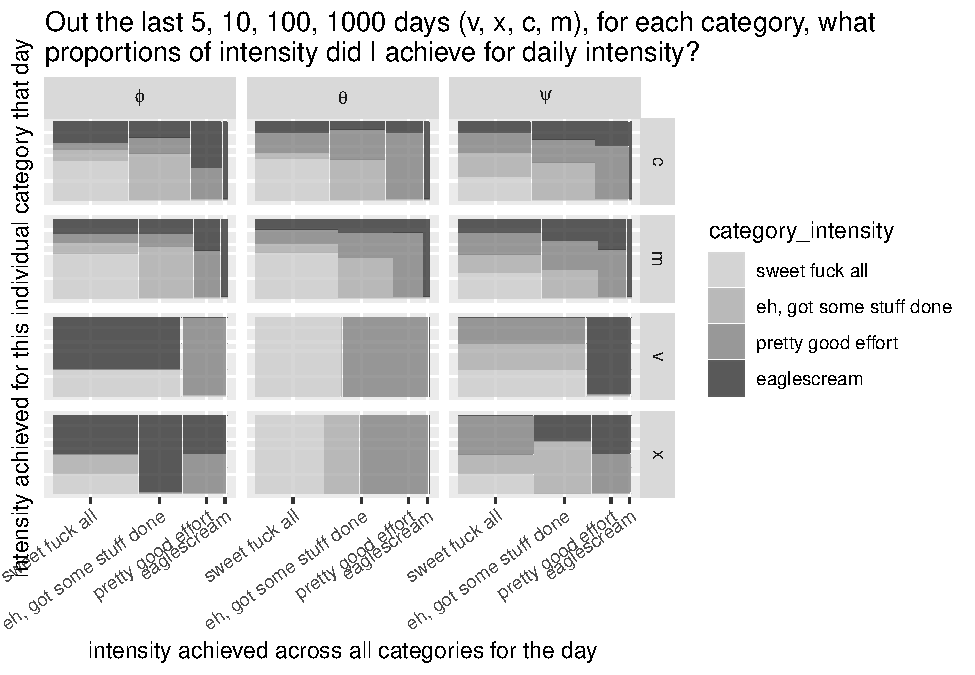
\includegraphics{lifeswork_files/figure-latex/intensity mosaic-1.pdf}

\hypertarget{distribution-of-work}{%
\section{distribution of work}\label{distribution-of-work}}

\begin{Shaded}
\begin{Highlighting}[]
\NormalTok{category_boxplot}
\end{Highlighting}
\end{Shaded}

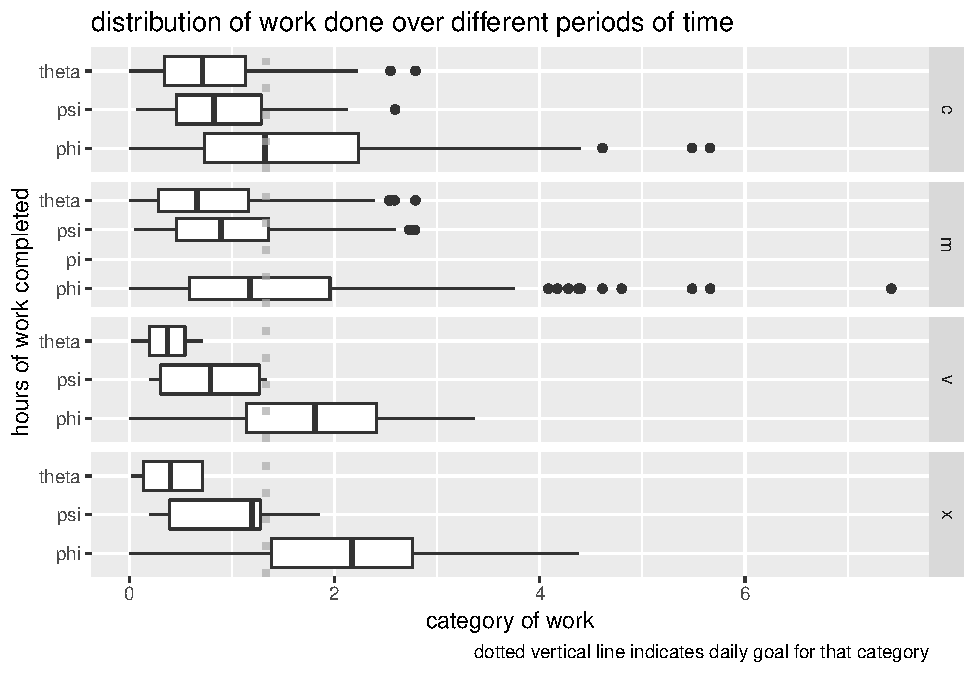
\includegraphics{lifeswork_files/figure-latex/category boxplot-1.pdf}

\hypertarget{rituals}{%
\chapter{rituals}\label{rituals}}

\begin{Shaded}
\begin{Highlighting}[]
\CommentTok{# packages used in this chapter}
\KeywordTok{library}\NormalTok{(dontpanic)}
\KeywordTok{library}\NormalTok{(tidyverse)}
\KeywordTok{library}\NormalTok{(googlesheets)}
\end{Highlighting}
\end{Shaded}

\begin{Shaded}
\begin{Highlighting}[]
\CommentTok{# register sheet}
\NormalTok{measures <-}\StringTok{ }\KeywordTok{gs_key}\NormalTok{(measures_gs_key)}

\CommentTok{# should extract the ws read for just}
\CommentTok{# wrangling}
\NormalTok{daily_tasks <-}\StringTok{ }\KeywordTok{get_daily_tasks}\NormalTok{()}
\NormalTok{workload_key <-}\StringTok{ }\KeywordTok{get_workload_key}\NormalTok{()}

\CommentTok{# better to pipe gs read into a wrangling function}

\NormalTok{signifiers <-}\StringTok{ }\NormalTok{measures }\OperatorTok\StringTok{ }\KeywordTok{gs_read}\NormalTok{(}\StringTok{"signifiers"}\NormalTok{)}
\NormalTok{day_view <-}\StringTok{ }\NormalTok{measures }\OperatorTok\StringTok{ }\KeywordTok{gs_read}\NormalTok{(}\StringTok{"day_view"}\NormalTok{)}
\end{Highlighting}
\end{Shaded}

\hypertarget{instantiate}{%
\section{instantiate}\label{instantiate}}

Ask albert to instantiate.

♪ top of today's \protect\hyperlink{daily-log}{daily log} and \protect\hyperlink{dayview:day-view}{day view}.

Date with

\begin{Shaded}
\begin{Highlighting}[]
\KeywordTok{today_date}\NormalTok{() }\OperatorTok\StringTok{ }\KeywordTok{cat}\NormalTok{()}
\end{Highlighting}
\end{Shaded}

\begin{verbatim}
## la date d'aujourd'hui est dimanche, vingt-six mai
\end{verbatim}

pic.twitter.com/wrCNDIcdLt

--- Charles T. Gray (\citet{cantabile}) May 26, 2019

Draw up \protect\hyperlink{dayview:day-view}{day view}.

In ♪ daily log, add priority daily tasks \(*\) ♪ \(+ \psi\), with \(*\) ♪ added to \protect\hyperlink{dayview:day-view}{projects}.

In 𝄐 \protect\hyperlink{dayview:day-view}{waiting}, schedule other \protect\hyperlink{daily-tasks}{daily tasks} ♪ \(\sim \varnothing\).

Add \textgreater{} \(*+\pi\cdot\) \protect\hyperlink{housework}{housework} \(\sharp\) tasks and \(\sharp \pi \cdot\) coffee to ♪ daily log. You deserve it.

Add \protect\hyperlink{review}{\(\overline o\)} and \(\pi\) to the \protect\hyperlink{dayview:order-of-events}{order of events}.

pic.twitter.com/yEKIgDcBGE

--- Charles T. Gray (\citet{cantabile}) May 26, 2019

\hypertarget{dayview:day-view}{%
\section{day view}\label{dayview:day-view}}

\begin{Shaded}
\begin{Highlighting}[]
\NormalTok{day_view }\OperatorTok\StringTok{ }
\StringTok{  }\CommentTok{# create links}
\StringTok{  }\KeywordTok{mutate}\NormalTok{(}\DataTypeTok{tracker =} \KeywordTok{paste0}\NormalTok{(}\StringTok{"["}\NormalTok{, tracker, }\StringTok{"]("}\NormalTok{,ref,}\StringTok{")"}\NormalTok{)) }\OperatorTok\StringTok{ }
\StringTok{  }\KeywordTok{select}\NormalTok{(}\OperatorTok{-}\NormalTok{ref) }\OperatorTok\StringTok{ }
\StringTok{  }\KeywordTok{lifeswork_table}\NormalTok{()}
\end{Highlighting}
\end{Shaded}

tracker

position

description

\href{dayview:goals}{goals}

top left

pom goals

\href{dayview:order-of-events}{order of events}

below goals

top row plans alternation of \(\cdot\) and \(pi\); now incorporates events

\href{dayview:pom-tracker}{pom tracker}

between goals and projects

count how many poms have been achieved per category

\href{dayview:projects}{projects}

top right

active projects: one per category

\href{dayview:task-cycles}{task cycles}

below order of events

plan upcoming task cyles

\href{dayview:progressed}{projects progressed}

below pom tracker

monthly log projects progressed today

\href{dayview:waiting}{waiting}

below projects progressed

for paring down to three active projects

pic.twitter.com/yEKIgDcBGE

--- Charles T. Gray (\citet{cantabile}) May 26, 2019

\hypertarget{daily-tasks}{%
\section{daily tasks}\label{daily-tasks}}

\begin{Shaded}
\begin{Highlighting}[]
\NormalTok{wrangle_tasks <-}\StringTok{ }\ControlFlowTok{function}\NormalTok{(tasks)\{}
\NormalTok{  tasks }\OperatorTok\StringTok{ }
\StringTok{  }\KeywordTok{mutate}\NormalTok{(}\DataTypeTok{priority =} \KeywordTok{map_chr}\NormalTok{(priority, knittify_latex),}
         \DataTypeTok{context =} \KeywordTok{map_chr}\NormalTok{(context, knittify_latex),}
         \DataTypeTok{category =} \KeywordTok{map_chr}\NormalTok{(category, knittify_latex)) }\OperatorTok\StringTok{ }
\StringTok{  }\KeywordTok{lifeswork_table}\NormalTok{()}
\NormalTok{\}}
\end{Highlighting}
\end{Shaded}

\hypertarget{section}{%
\subsection{\texorpdfstring{\(*\)}{*}}\label{section}}

priority

context

category

task

description

\(\star\)

\(\natural\)

\(\psi\)

calendar

check day, week, month; note events of the day; upcoming deadlines

\(\star\)

\(\forall\)

\(\psi\)

what is on fire?

task or project must be due today and someone else will get stuffed around if I don't do it

\(\star\)

\(\natural\)

\(\psi\)

email inbox

label as needs-action, waiting, archive

\(\star\)

\(\natural\)

\(\psi\)

3c\^{}2 inbox

NA

\(\star\)

\(\sharp\)

\(\pi\)

unpack suitcase

NA

\(\star\)

\(\sharp\)

\(\psi\)

pill

take medication

\(\star\)

\(\sharp\)

\(\pi\)

kitchen

clean kitchen

\(\star\)

\(\sharp\)

\(\pi\)

laundry

put away one basket of laundry

\(\star\)

\(\sharp\)

\(\pi\)

floors

vacuum or sweep living area

\hypertarget{housework}{%
\subsection{\texorpdfstring{\(* \sharp\)}{* \textbackslash{}sharp}}\label{housework}}

\begin{Shaded}
\begin{Highlighting}[]
\NormalTok{daily_tasks }\OperatorTok\StringTok{ }
\StringTok{  }\KeywordTok{filter}\NormalTok{(}\KeywordTok{str_detect}\NormalTok{(.}\OperatorTok{$}\NormalTok{category, }\StringTok{"pi"}\NormalTok{),}
         \KeywordTok{str_detect}\NormalTok{(.}\OperatorTok{$}\NormalTok{context, }\StringTok{"sharp"}\NormalTok{)) }\OperatorTok\StringTok{ }
\StringTok{  }\KeywordTok{wrangle_tasks}\NormalTok{()}
\end{Highlighting}
\end{Shaded}

priority

context

category

task

description

\(\varnothing\)

\(\sharp\)

\(\pi\)

handbag

NA

\(\star\)

\(\sharp\)

\(\pi\)

unpack suitcase

NA

\(\varnothing\)

\(\sharp\)

\(\pi\)

wash brushes

wash brushes

\(\star\)

\(\sharp\)

\(\pi\)

kitchen

clean kitchen

\(\star\)

\(\sharp\)

\(\pi\)

laundry

put away one basket of laundry

\(\star\)

\(\sharp\)

\(\pi\)

floors

vacuum or sweep living area

\(\varnothing\)

\(\sharp\)

\(\pi\)

water plants

NA

\(\varnothing\)

\(\sharp\)

\(\pi\)

vacuum

the other areas

\hypertarget{sim}{%
\subsection{\texorpdfstring{\(\sim\)}{\textbackslash{}sim}}\label{sim}}

\begin{Shaded}
\begin{Highlighting}[]
\NormalTok{daily_tasks }\OperatorTok\StringTok{ }
\StringTok{  }\KeywordTok{filter}\NormalTok{(priority }\OperatorTok{==}\StringTok{ "sim"}\NormalTok{) }\OperatorTok\StringTok{ }
\StringTok{  }\KeywordTok{wrangle_tasks}\NormalTok{()}
\end{Highlighting}
\end{Shaded}

priority

context

category

task

description

\(\sim\)

\(\natural\)

\(\psi\)

needs action

finish pom

\(\sim\)

\(\forall\)

\(\psi\)

monthly log

each project should either have an associated collection, or a git hub repo or issue, location tagged in monthly log

\(\sim\)

\(\natural\)

\(\psi\)

ynab

finish pom

\(\sim\)

\(\forall\)

\(\psi\)

thread

NA

\hypertarget{varnothing}{%
\subsection{\texorpdfstring{\(\varnothing\)}{\textbackslash{}varnothing}}\label{varnothing}}

\begin{Shaded}
\begin{Highlighting}[]
\NormalTok{daily_tasks }\OperatorTok\StringTok{ }
\StringTok{  }\KeywordTok{filter}\NormalTok{(priority }\OperatorTok{==}\StringTok{ "varnothing"}\NormalTok{,}
\NormalTok{         category }\OperatorTok{!=}\StringTok{ "pi"}\NormalTok{) }\OperatorTok\StringTok{ }
\StringTok{  }\KeywordTok{wrangle_tasks}\NormalTok{()}
\end{Highlighting}
\end{Shaded}

priority

context

category

task

description

\(\varnothing\)

\(\natural\)

\(\theta\)

export measures

download report into files, then email to myself, then download

\(\varnothing\)

\(\natural\)

\(\psi\)

waiting

waiting emails

\hypertarget{pi}{%
\subsection{\texorpdfstring{\(\pi\)}{\textbackslash{}pi}}\label{pi}}

\begin{Shaded}
\begin{Highlighting}[]
\NormalTok{daily_tasks }\OperatorTok\StringTok{ }
\StringTok{  }\KeywordTok{filter}\NormalTok{(category }\OperatorTok{==}\StringTok{ "pi"}\NormalTok{) }\OperatorTok
\StringTok{  }\KeywordTok{wrangle_tasks}\NormalTok{()}
\end{Highlighting}
\end{Shaded}

priority

context

category

task

description

\(\varnothing\)

\(\sharp\)

\(\pi\)

handbag

NA

\(\star\)

\(\sharp\)

\(\pi\)

unpack suitcase

NA

\(\varnothing\)

\(\natural\)

\(\pi\)

write to dani

check in with dani on slack

\(\varnothing\)

\(\sharp\)

\(\pi\)

wash brushes

wash brushes

\(\star\)

\(\sharp\)

\(\pi\)

kitchen

clean kitchen

\(\star\)

\(\sharp\)

\(\pi\)

laundry

put away one basket of laundry

\(\star\)

\(\sharp\)

\(\pi\)

floors

vacuum or sweep living area

\(\varnothing\)

\(\sharp\)

\(\pi\)

water plants

NA

\(\varnothing\)

\(\sharp\)

\(\pi\)

vacuum

the other areas

\hypertarget{email}{%
\section{email}\label{email}}

\hypertarget{process-inbox}{%
\subsection{process inbox}\label{process-inbox}}

Check inbox once a day.

\begin{itemize}
\tightlist
\item
  archive {[}and label{]} emails that don't require actions
\item
  if I know what I want to say, best to do it now
\item
  if it's going to be lengthy or \(\sim\), label as \texttt{needs\ action}
\end{itemize}

\hypertarget{needs-action}{%
\subsection{needs action}\label{needs-action}}

\begin{itemize}
\tightlist
\item
  start from the bottom, gmail doesn't sort descending
\item
  write a next action
\item
  migrate task to \(\sim\) {[}todo: quaver{]} \(+ \sim\)
\item
  can stop after one pom on this each day
\end{itemize}

\hypertarget{review}{%
\section{\texorpdfstring{\textbf{\texttt{review}}}{review}}\label{review}}

\hypertarget{dayview:daily-log}{%
\subsection{daily log}\label{dayview:daily-log}}

This is the hard part.

Pare down to one active project per category and process daily list to end of log.

Cross through actions above.

\hypertarget{if-this-project-will-take-more-than-a-day}{%
\subsubsection{if this project will take more than a day}\label{if-this-project-will-take-more-than-a-day}}

\begin{itemize}
\item
  if (\(*\)) or (\(\sim\)), create project for next step and migrate to projects waiting to progress
\item
  else if associated with a repo, migrate to issues
\item
  else migrate to \protect\hyperlink{monthly-log}{monthly log}
\item
  add \protect\hyperlink{signifiers}{signifiers}
\item
  log projects in \protect\hyperlink{day-view}{day view} tracker
\item
  add projects from \protect\hyperlink{monthly-log}{monthly log} if all \(*\) and \(\sim\) have been completed
\item
  aim to progress at least one \(*\) from the \protect\hyperlink{monthly-log}{monthly log}
\end{itemize}

\hypertarget{day-view}{%
\subsection{day view}\label{day-view}}

This is the sparkjoy bit.

\begin{itemize}
\tightlist
\item
  count poms
\item
  log goals
\item
  top up projects from \protect\hyperlink{projects-waiting}{projects waiting} to maximum three active projects, one per category
\item
  assign task cycles

  \begin{itemize}
  \tightlist
  \item
    exclude \(\varnothing\) categories with no \(*\) and \(\sim\) projects where current goal has already been met in poms by category
  \item
    always finish with scheduling review \(\overline o\)
  \item
    consider including a \href{https://en.wikipedia.org/wiki/Marie_Kondo}{sparkjoy} project
  \end{itemize}
\item
  calculate remaining poms
\end{itemize}

\hypertarget{assess}{%
\subsection{assess}\label{assess}}

plan poms and \(\pi\) to next goal

Calculate number of poms I can realistically do, the floor of
\[
14 - t - \frac 3 2 c
\]
where \(t\) denotes the number of hours of travel, and \(c\) the number of hours of \emph{community}, where the lattter includes teaching, outreach, and research collaborations. That, is I aim to draw a distinction between self-directed time, and time where I have the benefit of external motivations.

\begin{Shaded}
\begin{Highlighting}[]
\CommentTok{# todo: import tidyverse into dontpanic}

\KeywordTok{library}\NormalTok{(tidyverse)}

\CommentTok{# output as of this update}

\CommentTok{# todo: add dataset arg to fn}

\NormalTok{dontpanic}\OperatorTok{::}\KeywordTok{calculate_pom_goal}\NormalTok{(}
  \DataTypeTok{travel_hrs =} \DecValTok{0}\NormalTok{, }\CommentTok{# no travel today}
  \DataTypeTok{community_hrs =} \DecValTok{0} \CommentTok{# no teaching, meetings today}
\NormalTok{)}
\end{Highlighting}
\end{Shaded}

\begin{verbatim}
## 
## aim to get 14 poms done today
\end{verbatim}

\begin{verbatim}
## # A tibble: 9 x 5
##   workload usual category  poms pom_diff
##   <chr>    <dbl> <chr>    <dbl>    <dbl>
## 1 light        4 phi          2        2
## 2 moderate     8 phi          4        4
## 3 hardcore    14 phi          6        6
## 4 light        4 theta        1        1
## 5 moderate     8 theta        2        2
## 6 hardcore    14 theta        4        4
## 7 light        4 psi          1        1
## 8 moderate     8 psi          2        2
## 9 hardcore    14 psi          4        4
\end{verbatim}

\hypertarget{minibreak-peeps}{%
\subsection{minibreak peeps}\label{minibreak-peeps}}

\begin{itemize}
\tightlist
\item
  social media \& slack
\end{itemize}

\hypertarget{task-cycle}{%
\section{task cycle}\label{task-cycle}}

\begin{longtable}[]{@{}ll@{}}
\toprule
shorthand & description\tabularnewline
\midrule
\endhead
\(\forall *\) & complete all priority (\(*\)) tasks\tabularnewline
\(\sim \geqslant 1\) & complete at least one anxiety (\(\sim\)) task\tabularnewline
\(\varnothing \geqslant 0\) & complete any or none of the untagged tasks\tabularnewline
\(\cdot \geqslant 1\) & write down as many next actions as I can think of\tabularnewline
\(\overline o\) & \protect\hyperlink{review}{review}\tabularnewline
\bottomrule
\end{longtable}

\hypertarget{monthly-log}{%
\section{monthly log}\label{monthly-log}}

List of projects that will take longer than a day.

Need to incorporate this into managing papers.

Chatting to a colleague and told them about the 30:80 model of writing a manuscript that I find really useful - thought I'd share it here to see if anyone else had something similar\ldots{}? \#writing \#academicwriting (1/7)

--- Neal Haddaway (\citet{nealhaddaway}) May 6, 2019

\hypertarget{dayview:goals}{%
\section{pom goals}\label{dayview:goals}}

pom := 20 minutes

pic.twitter.com/MGRLiYviCX

--- Charles T. Gray (\citet{cantabile}) May 26, 2019

\hypertarget{dayview:pom-tracker}{%
\section{pom tracker}\label{dayview:pom-tracker}}

\hypertarget{dayview:projects}{%
\section{projects}\label{dayview:projects}}

\hypertarget{dayview:task-cycles}{%
\section{task cycles}\label{dayview:task-cycles}}

\hypertarget{dayview:progressed}{%
\section{♫ progressed}\label{dayview:progressed}}

\hypertarget{dayview:waiting}{%
\section{waiting}\label{dayview:waiting}}

\hypertarget{dayview:order-of-events}{%
\section{order of events}\label{dayview:order-of-events}}

Day begins with \protect\hyperlink{review}{review} \(\overline o\).

\hypertarget{workday}{%
\subsection{workday}\label{workday}}

Alternate events:

\begin{itemize}
\tightlist
\item
  \(\not n + 2\) poms
\item
  \(\pi\)
\end{itemize}

Around other events such as meetings.

\hypertarget{wake-up}{%
\subsection{wake up}\label{wake-up}}

\begin{itemize}
\tightlist
\item
  wake up
\item
  {[}read{]}
\item
  wash \& dress
\item
  {[}yoga{]}
\item
  \protect\hypertarget{day-view}{}{day view}
\item
  {[}yoga{]}
\end{itemize}

\hypertarget{evening}{%
\subsection{evening}\label{evening}}

\begin{itemize}
\tightlist
\item
  bathtime + reading
\item
  bed
\end{itemize}

\hypertarget{signifiers}{%
\section{signifiers}\label{signifiers}}

\begin{quote}
todo: create a signifiers sheet
\end{quote}

signifier

meaning

position

\(\eigthnote\)

today

4

\(star\)

priority

5

\(i, ii, \dots\)

project

4

\(sim\)

anxiety

5

\(\cdot\)

task

1

\(\varphi\)

research

2

\(\theta\)

skills

2

\(psi\)

busywork

2

\(NA\)

project

3

\(NA\)

look into

3

\(\natural\)

on computer

2

\(o\)

event

1

\(\overline o\)

review

1

\(NA\)

more than a day

2

\hypertarget{playlists}{%
\section{playlists}\label{playlists}}

\hypertarget{for-the-good-days}{%
\subsection{for the good days}\label{for-the-good-days}}

\hypertarget{for-the-not-so-good-days}{%
\subsection{for the not so good days}\label{for-the-not-so-good-days}}

\hypertarget{ruminations}{%
\chapter{ruminations}\label{ruminations}}

\hypertarget{daily-projects}{%
\section{daily projects}\label{daily-projects}}

If a project is logged in the \protect\hypertarget{daily-log}{}{daily-log} then I am committing to finishing it today.

\hypertarget{pomodoros}{%
\section{pomodoros}\label{pomodoros}}

20 minutes seems to be the amount of time I can reasonably expect myself to focus unbroken.

\hypertarget{lowtech}{%
\section{lowtech}\label{lowtech}}

Keep what can be kept on paper, on paper. Keeps screens free of clutter and helps me focus.

\hypertarget{work-with-intent}{%
\section{work with intent}\label{work-with-intent}}

This term is adopted from a piano teacher that I studied under, that I subsequently adapted into my own teaching. She encouraged me to \emph{practice with intent}; that is, play what you intend to play. I found this to be particularly useful for discouraging my students, and myself, from the age-old pitfall of playing a piece of music until you make a mistake and stopping and playing that section over until you get it right. It's better to play \emph{through} the piece, which empowers you to adapt to mistakes you will inevitably play and, most importantly, not lose time. Oddly, it appeared to be a universal misconception, myself included, that without careful consideration, the attempt to \emph{get the notes right} inevitably means the \textbf{rhythm is wrong}, and thus you get nothing right after all. Best, therefore, to play through the piece. I use my bullet journal to help me focus on work with intent; I've found the simplicity of only timing work when I've written down what I intend to do has been extraordinarily powerful in helping me complete daunting tasks.

\hypertarget{mindfulness}{%
\section{documenting the system is mindful time}\label{mindfulness}}

I often update my system. I see this as productive mindfulness; it is both meditative, I enjoy making something I find aesthetically pleasing, and functional, the systems do help me work happier.

Something that really resonated with me about Cal Newport's \emph{Deep Work} was that my situation will change, and so, too, may what best facillitates flow. I will pick and choose elements from pomodoro, gtd, task switching, and so forth to achieve flow. Allowing this to be so flexible makes keeping track of my own system tricky at times.

todo: fix inconsistencies in audience across manuscript - should be to self

I am slowly automating the process of updates, where the manual process is ideally kept to tweaking a set of easy to navigate \href{https://docs.google.com/spreadsheets/d/1hv7pkBGu8XQQOIBbBt1_1LvKGBR7zTdQYCzogrv3hz0/edit?usp=sharing}{googlesheets} which are scraped using the fabulous \texttt{googlesheets::} and rendered with \texttt{bookdown::}. It's exciting that using git, I can examine past systems.

todo: refs

This has a dual objective of providing a place to drop my thoughts, but also to test run \texttt{bookdown::}, as I will likely write my thesis in something this or \texttt{distill::}. Also, I think it'll level up my git-surfing skills.

I enjoy taking breaks from doing mathematics to document my system and analyse my productivity.

I often feel like it's about finding activities that are posisitive experiences \emph{and} productive in some way (for me, \(\varphi\), \(\theta\), \(\psi\), andn \(\pi\)). So, working on my system is \(\pi\).

\hypertarget{sim-beethoven-piano-sonata}{%
\section{\texorpdfstring{\(\sim\) beethoven piano sonata}{\textbackslash{}sim beethoven piano sonata}}\label{sim-beethoven-piano-sonata}}

todo:
\url{https://twitter.com/cantabile/status/1112145903203180544}

\bibliography{book.bib,packages.bib}


\end{document}
